\subsection{Recurrent neural network} % 2.5 pages
CNN solves the spatial problem of imagery and has been widely used in the field of computer vision, but it is powerless for data with time-series features.
For example, it is necessary to understand the words sequentially in sentences in natural language processing tasks.
And in understanding videos, it is necessary to understand the relationship between frames.
In these tasks, a recurrent neural network (RNN) is essential to process the time-series features.

\citet{jordan1986serial} proposes the Jordan network, by introducing a recurrent connection that feeds back the output of the whole network to the input layer after a time delay. 
Later in 1990, \citet{elman1990finding} formally defines the RNN model.
The output of each recurrent layer sends to the subsequent layers and feeds back to the input of the layer after a time delay.

\begin{figure}[ht!]
    \centering
    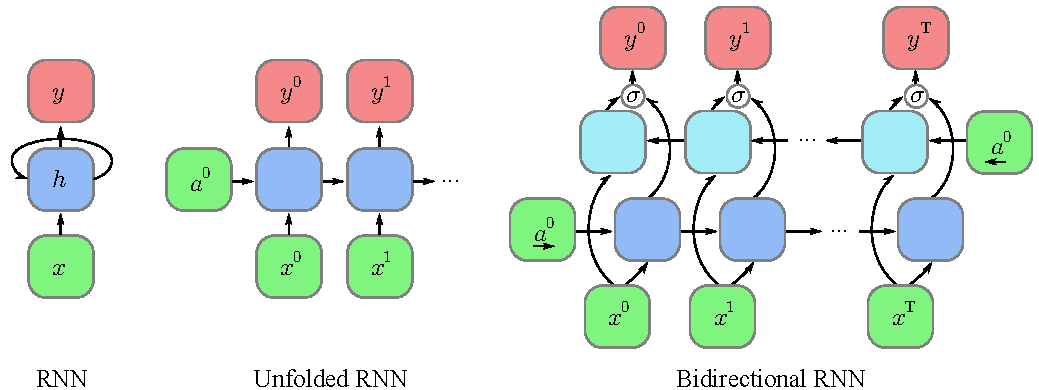
\includegraphics[width=\textwidth]{literature/imgs/2-RNN-unfold.pdf}
    \caption{RNN structure unfolded and bidirectional RNN}
    \label{fig:2-RNN-unfold}
\end{figure}

%LSTM
\citet{hochreiter1997long}

% RNN & LSTM fundamentals summary
\citet{sherstinsky2020fundamentals}

%GRU
\citet{chung2014empirical}

\begin{figure}[ht!]
    \centering
    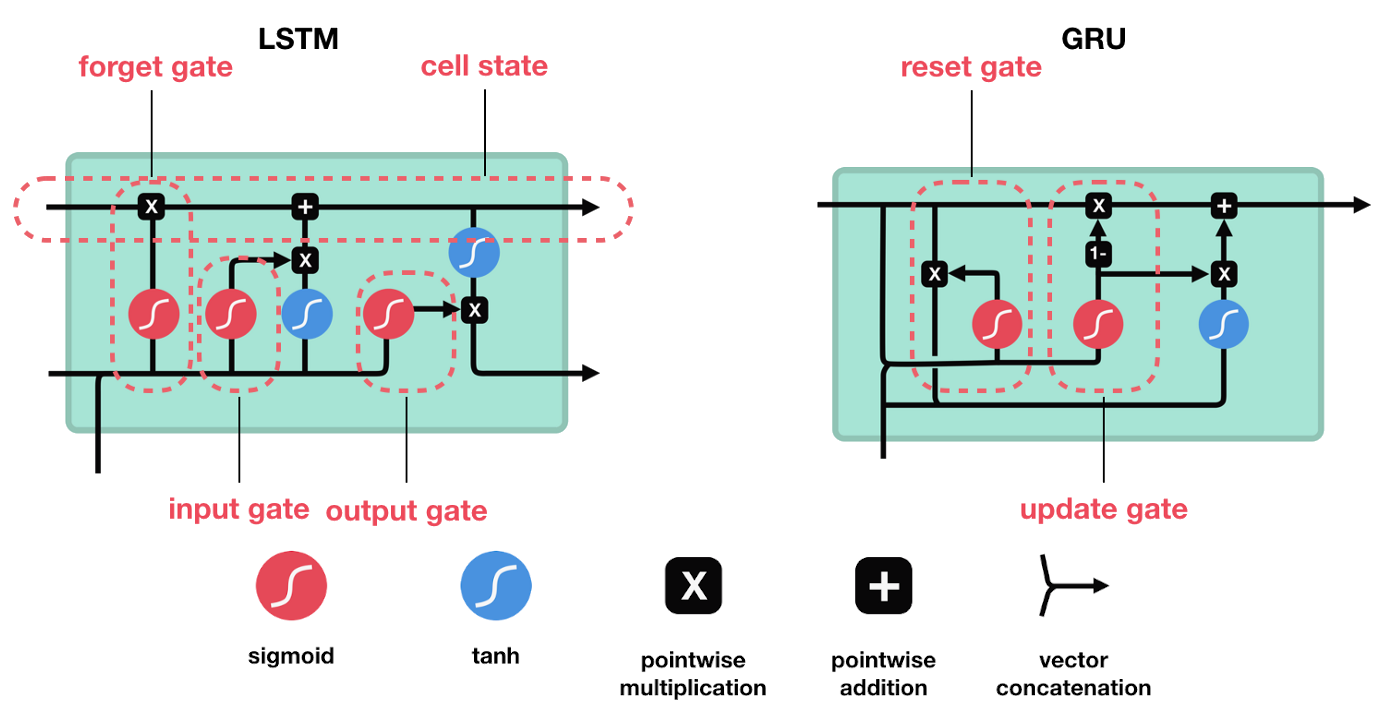
\includegraphics[width=.9\textwidth]{literature/imgs/ext-LSTM-GRU.png}
    \caption{LSTM and GRU structure comparison by \citet{phi2018illustrated}}
    \label{fig:ext-LSTM-GRU}
\end{figure}

Sequential computing restriction and long-term memory loss issues.